\documentclass[a4paper,11pt]{article}

\usepackage[T1]{fontenc}
\usepackage[utf8]{inputenc}
\usepackage[english,polish]{babel}
\usepackage{lmodern}
\usepackage{graphicx}
\usepackage{fancyhdr}
\usepackage{float}
\usepackage{array}

%\usepackage{mathtools}


\setlength{\textheight}{23.5cm}
\setlength{\textwidth}{15.92cm}
\setlength{\footskip}{10mm}
\setlength{\oddsidemargin}{0mm}
\setlength{\evensidemargin}{0mm}
\setlength{\topmargin}{0mm}
\setlength{\headsep}{15mm}
\setlength{\parindent}{0cm}
\setlength{\parskip}{2.5mm}
\author{Justyna Ilczuk, Jacek Rosiński}

\begin{document}

\begin{center}

    \begin{tabular}{ | m{5cm}| m{5cm} | m{5cm} |}
    \hline 
    \multicolumn{2}{|c|}{Elektronika w eksperymencie fizycznym}
    & Rok akademicki 2012-2013 \\ 
    
    \hline
    Środa 14.15-17.00 
    & Justyna Ilczuk \newline Jacek Rosiński
    & Wykonane w dniu 17.04.2013 \\
   	
   	\hline
   	Ćwiczenie 8 & Elementy i układy przełączające &    Ocena: \\
   	\hline
    \end{tabular}
\end{center}

%\newpage
\pagestyle{fancy}
\fancyfoot[CO]{\ }
\fancyhead[RO]{\footnotesize{\thepage} }
%\fancyhead[RO]{\footnotesize{\ } }
\fancyhead[LO]{Justyna Ilczuk i Jacek Rosiński K-1, Elementy i układy przełączające }




\section{Cel ćwiczenia}
Celem ćwiczenia było poznanie parametrów przełączników elektryczych oraz zasad działania elektroniczych układów przełączających.

\section{Użyty sprzęt i układy pomiarowe}

Hardware:
\begin{itemize}
\item komputer PC
\item Elvis II+
\end{itemize}

Software:
\begin{itemize}
\item oprogramowanie od National Instruments do pomiarów na Elvisie

\end{itemize}

\subsection{Układy pomiarowe}

\section{Wstęp teoretyczny}


\section{Opracowanie wyników}
No więc, co nam wyszło?

\subsection{Badanie diod jako przełączników}
Na początku (w części pierwszej) badaliśmy układy przełączające z diodami, poniżej przedstawiamy zmierzone przebiegi dla częstotliwości 50 kHz.

Na poniższych rysunkach 1 kratka pozioma oznacza \(2 \mu s\).

W podpisach rysunków używamy \(E_F \) i \(E_R \) oraz \(U_{max} \)

\(U_{max} = E_F - E_R = 5V_{p-p}\)


Żeby się nie powtarzać: przy pomiarze czasów występuje niepewność, wynikająca z odczytu pomiaru, którą szacujemy na 1/10 podziałki, co w praktyce oznacza w przełożeniu na używane przez nas jednostki, że niepewność ta dla każdego odczytu czasu wynosi \(0.2 \mu s\).

Dla diody prostowniczej:

\begin{figure} [H]
  \begin{center}
    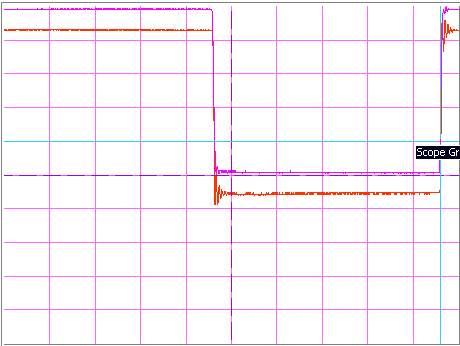
\includegraphics{../Obrazki_i_tekst/obrobione/1asciety.png}
    \caption{\( E_F = U_{max}, \ E_R = 0V \)}
  \end{center}
\end{figure}

Dla tego przypadku \( t_{off} \) praktycznie można pominąć, bo nie sposób wyznaczyć go na podstawie przebiegu.

\begin{figure} [H]
  \begin{center}
    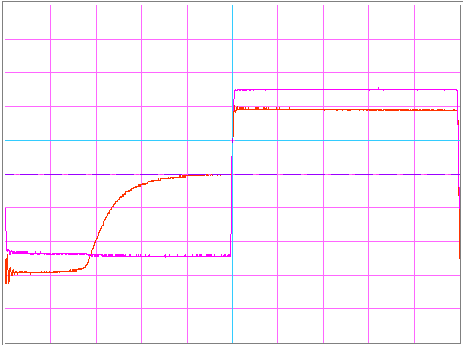
\includegraphics{../Obrazki_i_tekst/obrobione/1bsciety.png}
    \caption{\( E_F = 0.5 U_{max}, \ E_R = -0.5 U_{max}\)}
  \end{center}
\end{figure}

Gdy zmieniliśmy offset napięcia tak, że przełącznik był wyłączany napięciem - 2.5 V, sytuacja zdecydowanie się zmieniła i zaobserwowaliśmy następujące czasy wyłączania diody:

 \(t_1 = 3.6 \mu s,\ t_2 = 4.4 \mu s,\ t_{off} = 8 \mu s \).

\begin{figure} [H]
  \begin{center}
    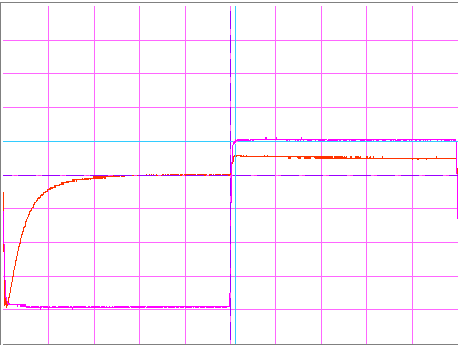
\includegraphics{../Obrazki_i_tekst/obrobione/1csciety.png}
    \caption{\( E_F = 1V, \ E_R = -4 V\)}
  \end{center}
\end{figure}

Dalej zmieniając offset, zauważamy, że charakterystyka przebiegu się zmienia i że t1, traci kosztem t2:

 \(t_1 = 0 \mu s,\ t_2 = 5 \mu s,\ t_{off} = 5 \mu s \).

\begin{figure} [H]
  \begin{center}
    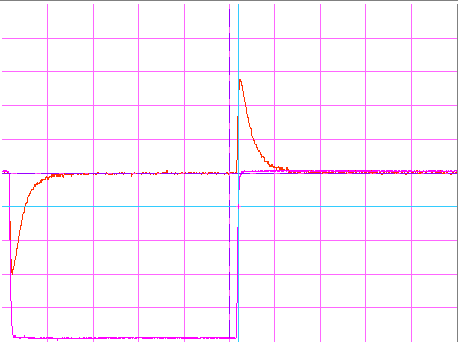
\includegraphics{../Obrazki_i_tekst/obrobione/1dsciety.png}
    \caption{\( E_F = 1V, \ E_R = -4 V\)}
  \end{center}
\end{figure}

Dalej zmieniając offset, tak że napięcie sterujące jest mniejsze, równe 0V, obserwujemy, że dioda nie zachowuje się uż jako przełącznik.

\begin{figure} [H]
  \begin{center}
    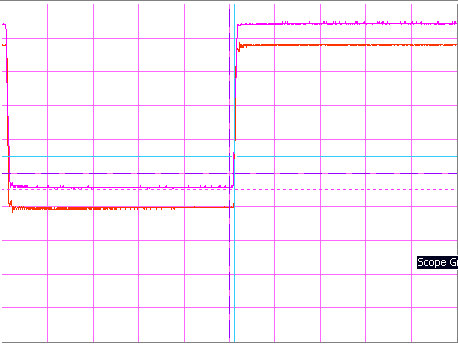
\includegraphics{../Obrazki_i_tekst/obrobione/1esciety.png}
    \caption{\( E_F = U_{max}, \ E_R = 0V \) z dołączonym kondensatorem \(C_L = 360 pF\)}
  \end{center}
\end{figure}

Ten układ różni się od pierwszego jedynie dołączonym kondensatorem \(C_L = 360 pF\). Nie dziwi zatem, że jego odpowiedź jest bardzo podobna do pierwszego układu, jeśli chodzi o różnice to, można zauważyć, że oscylacje na diodzie są mniejsze, ale poza tym jest praktycznie identycznie i czas wyłączania diody jest podobnie mały, tak że nie ma sensu go mierzyć.

Wszystkie poprzednie pomiary były przeprowadzone dla częstotliwości 50 kHz. Naszym kolejnym zadaniem było oszacowanie najmniejszej częstotliwości, przy której dioda przestaje pracować jako przełącznik.

\begin{figure} [H]
  \begin{center}
    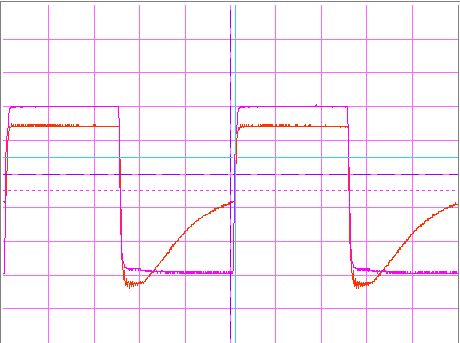
\includegraphics{../Obrazki_i_tekst/obrobione/2ciety.png}
    \caption{\( E_F = U_{max}, \ E_R = 0V \) dla częstotliwości 99 kHz }
  \end{center}
\end{figure}


Powyższy przebieg wyraźnie wskazuje, że dioda nie pracuje tu już jako przełącznik ponieważ cały czas płynie przez nią prąd w dwie strony i nie ma chwili, kiedy prąd przez nią nie płynie, czyli ani przez chwilę nie jest naprawdę wyłączona.

\textbf{Analogiczne badania przeprowadziliśmy dla diody impulsowej.}




\begin{figure} [H]
  \begin{center}
    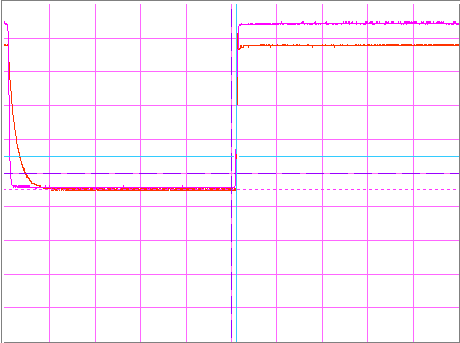
\includegraphics{../Obrazki_i_tekst/obrobione/31asciety.png}
    \caption{\( E_F = U_{max}, \ E_R = 0V \)}
  \end{center}
\end{figure}

Dla tego przypadku \( t_{off} \) jest stosunkowo niewielki.

\(t_1 = 0 \mu s,\ t_2 = 1.2 \mu s,\ t_{off} = 1.2 \mu s \).

\begin{figure} [H]
  \begin{center}
    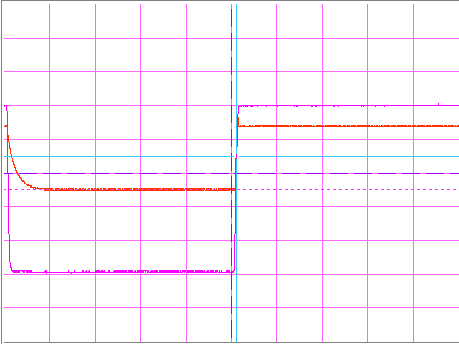
\includegraphics{../Obrazki_i_tekst/obrobione/31bsciety.png}
    \caption{\( E_F = 0.5 U_{max}, \ E_R = -0.5 U_{max}\)}
  \end{center}
\end{figure}

Gdy zmieniliśmy offset napięcia tak, że przełącznik był wyłączany napięciem - 2.5 V, czas wyłaczania diody praktycznie nie uległ zmianie:

\(t_1 = 0 \mu s,\ t_2 = 1.2 \mu s,\ t_{off} = 1.2 \mu s \).

\begin{figure} [H]
  \begin{center}
    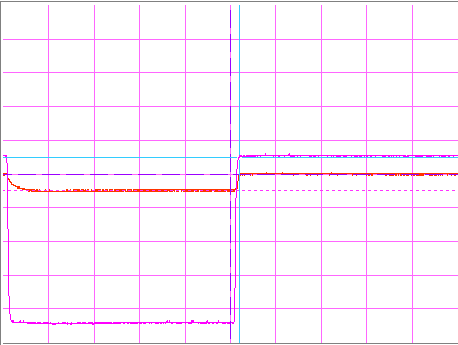
\includegraphics{../Obrazki_i_tekst/obrobione/31csciety.png}
    \caption{\( E_F = 1V, \ E_R = -4 V\)}
  \end{center}
\end{figure}

Dalej zmieniając offset, zauważamy, że zakres napięcia w którym przełącza dioda jest coraz mniejszy, czasy oszacowaliśmy następująco:

 \(t_1 = 0 \mu s,\ t_2 = 0.8 \mu s,\ t_{off} = 0.8 \mu s \).

\begin{figure} [H]
  \begin{center}
    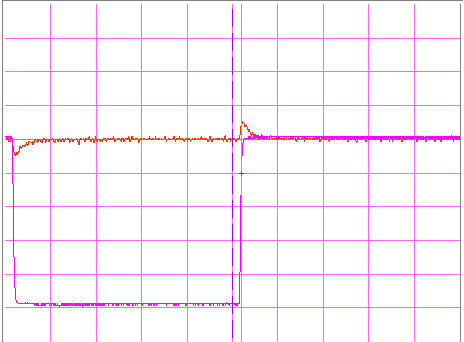
\includegraphics{../Obrazki_i_tekst/obrobione/31dsciety.png}
    \caption{\( E_F = 1V, \ E_R = -4 V\)}
  \end{center}
\end{figure}

Dalej zmieniając offset, tak że napięcie sterujące jest mniejsze, równe 0V, obserwujemy, że dioda nie zachowuje się uż jako przełącznik.

\begin{figure} [H]
  \begin{center}
    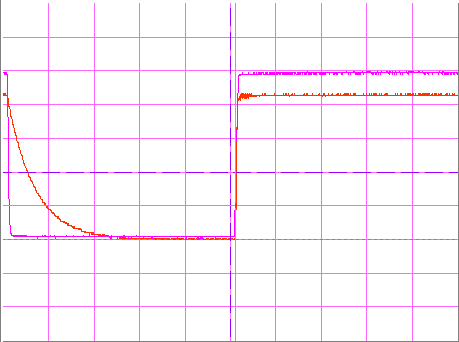
\includegraphics{../Obrazki_i_tekst/obrobione/31esciety.png}
    \caption{\( E_F = U_{max}, \ E_R = 0V \) z dołączonym kondensatorem \(C_L = 360 pF\)}
  \end{center}
\end{figure}

Ten układ różni się od pierwszego z diodą impulsową jedynie dołączonym kondensatorem \(C_L = 360 pF\). Jego odpowiedź jest bardzo podobna do pierwszego układu, ale czas \( t_2 \) zauważalnie się zwiększył.

\(t_1 = 0 \mu s,\ t_2 = 4 \mu s,\ t_{off} = 4 \mu s \).


\section{Niepewności}

% głównie cewki ... bo co innego + wzory 

\section{Wnioski}

% częstotliwości graniczne 
% uklady dobre w odpowiednich czestotliwosciach 
% od teraz zawsze bedziem cos włączać, bądź wyłączać, bo to kochamy ! 


\end{document}
